\documentclass[11pt]{article}
\usepackage[a4paper,margin=2.2cm]{geometry}
\usepackage{graphicx}
\usepackage{amsmath,amssymb}
\usepackage{booktabs,longtable,array}
\usepackage{hyperref}
\usepackage{caption}
\usepackage{microtype}
\usepackage{xcolor}
\usepackage{enumitem}
\setlist{nosep}
\hypersetup{colorlinks=true,linkcolor=black,urlcolor=blue,citecolor=black}
\begin{document}
\begin{center}
{\LARGE\bfseries Energy-Information Co-Design for Resource-Bounded Edge Intelligence: A Systems-Learning Federated Framework}\par\vspace{0.8em}
{\large Abhinandan Tripathi$^{1}$, Vijay Kumar Tiwari$^{2}$, Mohd. Arif$^{3}$, Abhishek Kumar Pandey$^{4,*}$, Shivam Bhardwaj$^{5}$}\par
$^{1}$Department of Computer Science and Engineering, Buddha Institute of Technology, Gorakhpur, India\par
$^{2}$Department of Information Technology, Madan Mohan Malaviya University of Technology (MMMUT), Gorakhpur, India\par
$^{3}$Department of Computer Science and Engineering, Galgotias University, Greater Noida, India\par
$^{4}$Department of Computer Science and Engineering, Bennett University, Greater Noida, India\par
$^{5}$United Institute of Management, Prayagraj, India\par
Emails: $^{1}$\href{mailto:abhinandan282@bit.ac.in}{abhinandan282@bit.ac.in}; $^{2}$\href{mailto:vktitca@mmmut.ac.in}{vktitca@mmmut.ac.in}; $^{3}$\href{mailto:md.arif@galgotiasuniversity.edu.in}{md.arif@galgotiasuniversity.edu.in};\par
$^{4}$\href{mailto:abhishek.pandey2@bennett.edu.in}{abhishek.pandey2@bennett.edu.in}; $^{5}$\href{mailto:shibambhardwaj@gmail.com}{shibambhardwaj@gmail.com}\par
ORCID: Abhishek Kumar Pandey — 0000-0003-3799-9754; Shivam Bhardwaj — 0009-0005-4554-7397\par
$^*$Corresponding author: Abhishek Kumar Pandey (\href{mailto:abhishek.pandey2@bennett.edu.in}{abhishek.pandey2@bennett.edu.in})\par
All authors contributed equally to this work.
\end{center}\vspace{0.8em}
\section*{Highlights}
\begin{itemize}
\item Network state is exposed directly to federated learning orchestration
\item Control-plane signaling is measured rather than assumed negligible
\item Matched controls reveal Pareto trade-offs between accuracy and relay cost
\item ns-3 replay links offered-load reduction to packet-network behavior
\end{itemize}
\section*{In brief}
Tripathi et al. frame federated edge intelligence as an energy-information co-design problem. Their controller coordinates utility-target participation, update fidelity, relay pressure, and staleness while explicitly pricing pre-selection signaling. Held-out real-data experiments and ns-3 low-power wireless replay expose workload-dependent Pareto trade-offs rather than universal dominance.\par
\section*{Broader context}
Resource-bounded edge intelligence increasingly supports environmental sensing, infrastructure observation, wearable analytics, and industrial monitoring. In these systems, selecting a learning client is also a physical resource-allocation decision because the selected update determines network load, relay burden, and delay. This study develops a systems-learning co-design framework that exposes multi-hop network state directly to federated orchestration. The evaluation deliberately separates learning gains from network costs, prices control metadata instead of treating scheduler information as free, and distinguishes open-loop packet replay from closed-loop co-simulation. The resulting evidence is best interpreted as a configurable Pareto mechanism for resource-bounded distributed AI rather than a universal efficiency or sustainability claim.\par
\section*{Abstract}
Resource-bounded edge intelligence is governed by a coupling that conventional learning-only optimization often hides: selecting a client determines not only which local information influences the model, but also how many bits must traverse the network, which routes and relays carry them, and whether delayed updates remain useful. We formulate this interaction as a systems-learning co-design problem and develop a hierarchical federated controller that exposes multi-hop network state directly to learning orchestration. The controller coordinates utility-target participation, route and residual-energy cost, relay-pressure feedback, adaptive Top-k update fidelity with error feedback, and utility-aware staleness weighting. The evaluation separates parameter tuning from held-out inference, corrects two-level aggregation-influence accounting, uses an overlap-safe blocked protocol for UCI HAR, and adds compression-matched controls plus a FedCG-adapted comparator. On Intel Berkeley Lab sensing data at strong resource-data correlation, the proposed controller achieves 1.7348 °C RMSE with 0.992 Mbit of model-update traffic. Resource-adaptive obtains lower RMSE and lower network cost, whereas the proposed controller reduces utility-target divergence by 86.0\%, exposing a genuine Pareto trade-off rather than universal dominance. On blocked UCI HAR, the proposed method reaches 88.67\% accuracy, 1.16 percentage points above resource-adaptive, while model-update traffic increases by 26.8\% and maximum relay energy by 628.9\%. Adaptive update fidelity reduces model-update traffic by 58.2\% on Intel and 64.0\% on HAR relative to the same scheduler at fixed 50\% Top-k. A conservative control-plane audit further shows that metadata cost is workload dependent: ETX-weighted pre-selection signaling is 1.219 Mbit on Intel and 0.306 Mbit on HAR. Even after this overhead is included, adaptive fidelity retains 38.4\% and 63.3\% control-inclusive uplink traffic reductions, respectively. Finally, ns-3.47 IEEE 802.15.4 replay demonstrates how reduced offered load changes delivery, delay, and channel contention. The evidence supports energy-information co-design as a configurable Pareto mechanism for resource-bounded distributed AI while distinguishing model-level gains from network-level costs and from claims requiring physical sensor-node validation.\par
Keywords: resource-bounded edge intelligence; energy-information co-design; distributed AI; federated learning; adaptive sparsification; network-aware learning; relay energy; staleness; edge-cloud systems.\par
\section{Introduction}
Edge intelligence is increasingly expected to operate where computation, communication capacity, and energy are simultaneously constrained. Environmental sensing, wearable intelligence, infrastructure monitoring, and industrial Internet-of-Things systems illustrate a common systems problem: the information that is most valuable for learning is not necessarily the information that is cheapest to acquire or transport. In distributed learning, client selection is therefore both a statistical decision and a physical resource-allocation decision.\par
This coupling is especially pronounced when model updates traverse multiple wireless hops before reaching an edge gateway. Selecting client i determines the local information entering training, but it also selects a route, an expected retransmission burden, intermediate relay activity, an arrival delay, and a contribution to future residual-energy imbalance. Treating communication as an independent transport service consequently hides an externality of distributed AI: statistically useful updates can be physically expensive, while inexpensive routes can repeatedly favor an easily reachable subset of clients.\par
We address this problem through systems-learning co-design. Rather than allowing the learning scheduler to optimize statistical utility while the network independently attempts to deliver the resulting updates, the proposed controller exposes route burden, residual-energy scarcity, relay pressure, update fidelity, and update age directly to learning orchestration. The resulting controller asks three coupled questions in each communication round: which eligible clients should participate, how much of each update should be retained, and how strongly should delayed information influence hierarchical aggregation?\par
This perspective differs from simply minimizing communication volume. A resource-only policy can reduce energy while narrowing the information entering training. A learning-only policy can repeatedly activate statistically useful but expensive routes and create relay hotspots. Adaptive sparsification introduces a third coupling because the retained update fraction changes both statistical fidelity and physical transmission burden. The relevant object is therefore a Pareto surface connecting predictive performance, communication demand, relay stress, and participation objectives rather than a single scalar notion of efficiency.\par
The present study deliberately treats ETX/residual-energy routing, hierarchy, sparsification, and staleness as established ingredients. Its contribution is the way these mechanisms are exposed to one another and audited under a common execution model. The revised evaluation is correspondingly conservative: the participation queue tracks a utility-derived target share rather than an externally defined population distribution, and the associated Jensen-Shannon divergence is therefore called utility-target alignment. Independent coverage diagnostics are reported separately. Cloud influence is also recorded only after both within-edge and cloud-level normalization.\par
The principal contributions are:\par
1. A systems-learning co-design formulation in which client participation prices multi-hop route burden, residual-energy scarcity, and relay-pressure externalities while retaining a utility-target participation-deficit term.\par
2. A client-specific finite-set Top-k fidelity rule with error feedback, coupled to the same network state that informs scheduling.\par
3. Correct two-level aggregation-influence accounting and an explicit separation between controller-target alignment, participation equality, and independent data-distribution coverage.\par
4. A measured control-plane audit that accounts for the bytes and a conservative radio-energy upper bound required to obtain pre-selection metadata instead of treating scheduler information as free.\par
5. A held-out evaluation protocol with disjoint tuning and evaluation seeds, compression-matched controls, a FedCG-adapted comparator, component ablations, exact paired statistical tests, and real sensing datasets.\par
6. Discrete-event ns-3.47 IEEE 802.15.4 replay that tests the packet-network consequences of the offered load produced by the learning/compression stack while explicitly distinguishing open-loop replay from closed-loop co-simulation.\par
The analytical and empirical evidence serve different purposes. Exact queue identities, finite-set compression decisions, top-k score selection, and error-feedback conservation are established for the implemented controller. By contrast, packet contention, acknowledgments, retransmissions, finite deadlines, and delayed arrivals are discrete systems phenomena that disappear when the network is reduced to a smooth communication penalty. We therefore use mathematical analysis where it applies exactly and executable network replay where the physical abstraction matters, rather than claiming a non-convex convergence theorem for a relaxed system that is not the one being executed.\par
\section{Related Work and Positioning}
Client-edge-cloud HFL was formalized by Liu et al. [1], and resource-aware client selection for IoT FL predates the present study [2]. Dynamic client-edge association and resource allocation have also been optimized jointly [3]. Long-term participation under volatile clients has been studied explicitly [4], while recent fairness-oriented analysis further distinguishes participation equality from distributional and performance fairness [13]. These results make hierarchy, multicriteria resource scoring, and participation-aware selection established ingredients rather than sufficient novelty claims.\par
Synchronization and heterogeneity have likewise been studied extensively. HiFlash couples adaptive staleness control with heterogeneity-aware client-edge association [5]. ShapeFL reduces communication by shaping edge-level data distributions [7], while cost-efficient HFL formulations jointly optimize selection and wireless resource allocation [8]. Recent graph-based HFL also combines client clustering with communication-resource allocation under non-IID data [17], learning-topology co-optimization has been studied for device-to-device HFL [18], and multi-job HFL jointly addresses client selection and resource allocation for consumer-grade UAVs [19]. Energy-efficient HFL has additionally been developed for marine IoT settings [20].\par
A related line of work focuses on selection diversity and compression. FedCG combines representative gradient-based client selection with adaptive compression [6]. Because its original communication model is not the multi-hop client-edge-cloud topology used here, we implement a clearly labeled FedCG-adapted comparator: a greedy facility-location selector over current client gradients with capability cost and adaptive compression. This is a favorable comparator because it has access to current gradient vectors for eligible clients; its information-acquisition overhead is not added to traffic accounting. It is not presented as an exact reproduction of FedCG.\par
Multi-hop FL itself is also established. Prior studies consider in-network aggregation with routing and spectrum allocation [9], network-accelerated FL over physical wireless edge systems [10], and multi-hop HFL grouping/resource allocation [11]. A topology-aware FL survey summarizes this broader design space [12]. The present work therefore does not claim novelty for ETX routing, multi-hop FL, fairness, compression, staleness, or hierarchy individually. Its research object is the joint control of utility-target participation, model-update fidelity, route burden, relay pressure, and staleness under a measured WSN substrate and held-out evaluation.\par
\section{System Model and Problem Definition}
Consider a WSN-IoT graph \(G=(\mathcal V,\mathcal E)\), a set of learning-capable clients \(\mathcal C\), edge gateways \(\mathcal G\), and a cloud server. Client \(i\) owns local data \(D\_i\sim P\_i(X,Y)\), where generally \(P\_i\neq P\_j\). At communication round \(t\), a binary variable \(x\_i(t)\) determines whether client \(i\) participates.\par
The network layer supplies a route \(\mathcal P\_i(t)\) from client \(i\) to an edge gateway. For link \((u,v)\), let \(\operatorname{ETX}\_{uv}(t)\) be its expected transmission count. Route burden is\par
\[
C_i^{\mathrm{route}}(t)=\sum_{(u,v)\in\mathcal P_i(t)}\operatorname{ETX}_{uv}(t).
\]
If \(b\_i(t)\) update bits are transmitted, expected traffic is\par
\[
B_i^{\mathrm{eff}}(t)=x_i(t)b_i(t)C_i^{\mathrm{route}}(t).
\]
Unlike a single-hop abstraction, the same update consumes energy on intermediate relays. The cumulative burden on relay \(r\) is\par
\[
E_r^{\mathrm{cum}}(T)=\sum_{t=1}^{T}\sum_i x_i(t)\mathbf 1[r\in\mathcal P_i(t)]E_{ir}^{\mathrm{relay}}(t).
\]
The learning problem is therefore not equivalent to selecting clients with minimum route cost. A high-loss or historically informative client can have a poor route, while cheap clients can dominate repeated selections. The controller is designed to expose rather than hide this trade-off.\par
Figure 1 is a conceptual systems schematic, not a prescribed physical deployment. The illustrated client-relay-edge-cloud branches communicate the hierarchy used by the controller; routing and scheduling operate on graph/network state rather than on a rigid geometric layout or a fixed floor plan.\par
\begin{figure}[htbp]
\centering
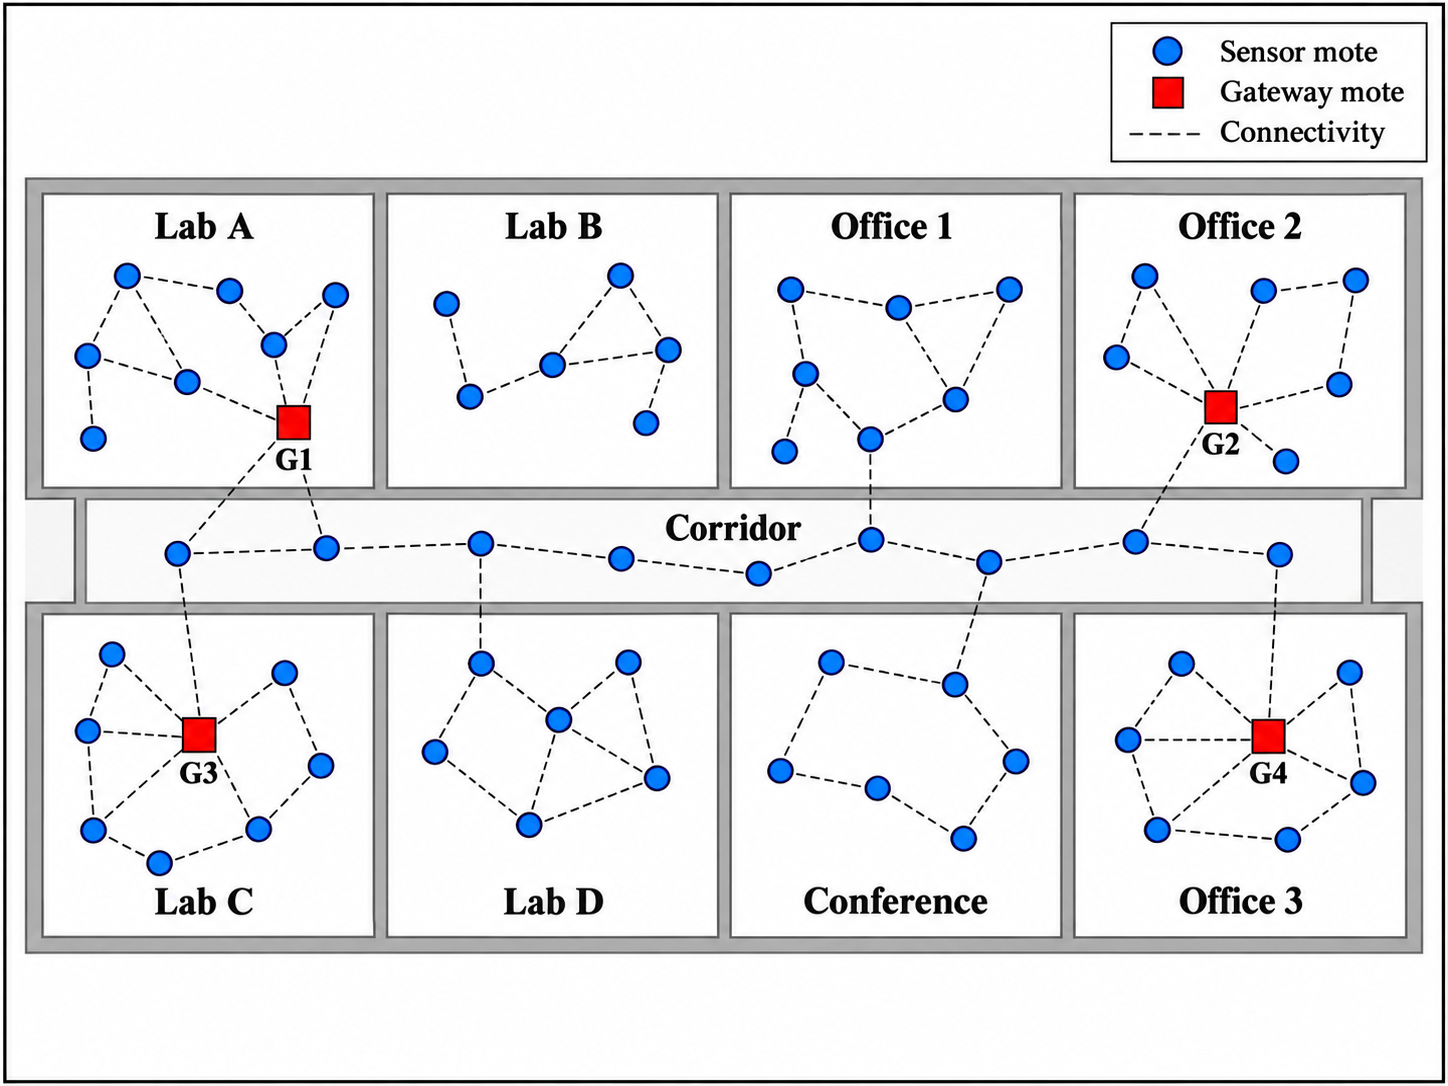
\includegraphics[width=0.96\linewidth]{figures/02_system_architecture.png}
\caption{Conceptual cross-layer HFL architecture. Learning-capable clients exchange models through multi-hop relays and edge gateways. Downlink dissemination is shown for system completeness; reported communication totals in this study refer to uplink model-update traffic unless stated otherwise.}
\end{figure}
\section{Systems-Learning Co-Design Controller}
\subsection*{Executed utility signal}
Conceptually, a client utility can contain novelty, learning difficulty, and distribution information:\par
\[
U_i(t)=\alpha_gG_i(t)+\alpha_lL_i(t)+\alpha_hH_i(t),
\]
where \(G\_i\) denotes update novelty, \(L\_i\) learning difficulty/progress, and \(H\_i\) an optional rarity term. The executed pre-selection utility is more specific: it is 0.55 times the per-round min-max-normalized current local loss plus 0.45 times the min-max-normalized exponentially smoothed utility history. No distribution-rarity term is used directly in the executed scheduling score. After a selected client trains, its history is updated from cosine novelty and non-negative local improvement. The improvement transform uses task-specific saturation constants documented in the repository. Raw examples remain local, but scalar loss/utility metadata are assumed available to the scheduler; this is not a formal privacy guarantee.\par
Throughout Sections 4-8, notation is fixed consistently. U\_i(t) denotes the executed pre-selection utility used by the target share and scheduling score; Q\_i(t) denotes the client participation-deficit queue; Z\_r(t) denotes relay-pressure state; and rho\_i(t) denotes the retained Top-k fraction, not the discarded fraction. The post-training novelty/improvement signal updates the smoothed utility history and the utility attached to the transmitted update; it is not substituted retrospectively into the pre-selection score.\par
The normalized desired utility-target participation share is\par
\[
\pi_i(t)=\frac{U_i(t)+\epsilon}{\sum_j(U_j(t)+\epsilon)}.
\]
\subsection*{Utility-target participation-deficit queue}
A virtual queue tracks the difference between desired and realized participation share:\par
\[
Q_i(t+1)=\left[Q_i(t)+\pi_i(t)-a_i(t)\right]^+.
\]
Here \(a\_i(t)=x\_i(t)/k\_t\) for a selected set of size \(k\_t>0\), and \(a\_i(t)=0\) when no client is selected. The mechanism does not enforce equal-frequency participation. Instead, persistent shortfall relative to the utility-derived target increases future scheduling pressure. Directly from the recursion,\par
\[
\frac1T\sum_{t<T}a_i(t) \ge \frac1T\sum_{t<T}\pi_i(t) - \frac{Q_i(T)-Q_i(0)}{T}.
\]
Rate stability of \(Q\_i\) is therefore sufficient for the long-run participation-share target. It does not prove equality between the target and final cloud influence, because compression, drops, staleness, edge normalization, and cloud normalization occur after selection.\par
\subsection*{Relay-pressure queue}
For relay \(r\), the controller maintains a virtual pressure queue relative to a relay-energy reference level:\par
\[
Z_r(t+1)=\left[Z_r(t)+E_r^{\mathrm{relay}}(t)-\bar E_r\right]^+,
\]
and route pressure for client \(i\) is\par
\[
R_i(t)=\sum_{r\in\mathcal P_i(t)}Z_r(t).
\]
The term increases when repeated model traffic funnels through the same relay corridor. In the executed policy, this relay-energy level is a pressure reference, not a hard per-round physical energy cap. The queue therefore biases future selections away from repeatedly stressed routes but does not by itself guarantee that a finite experiment will satisfy a strict cumulative relay budget.\par
\subsection*{Adaptive update fidelity}
Let \(\rho\_i(t)\) denote the retained Top-k fraction. The controller exhaustively evaluates the finite candidate set and minimizes\par
\[
J_i^{\mathrm{comp}}(\rho)= \rho\left(\widetilde C_i^{\mathrm{route}}+\eta_E\widetilde S_i+\eta_R\widetilde R_i\right) +\beta U_i(t)(1-\rho)^2.
\]
In the executed implementation, the scarcity term is the min-max-normalized value of max(initial-energy/residual-energy - 1, 0), and its coefficient eta\_E is fixed at 0.5. Route cost and relay pressure are also min-max normalized each round. The revised held-out protocol selects eta\_R = 5 and beta = 0.10 using tuning seeds only; the selection rule is described in Section 5.2. Error feedback carries omitted coordinates into later updates.\par
\subsection*{Queue-informed scheduling score}
For each eligible client,\par
\[
\Gamma_i(t)=V\widetilde U_i(t)+Q_i(t)-V\rho_i(t) \left(\widetilde C_i^{\mathrm{route}}+\eta_E\widetilde S_i+\eta_R\widetilde R_i\right).
\]
The executed controller uses eta\_E = 0.5, eta\_R = 5, and V = 0.5. If \(M\_t\) clients are eligible, it selects exactly \(k\_t=\min(K\_t,M\_t)\) clients with the largest \(\Gamma\_i(t)\). Eligibility uses availability and a residual-energy threshold; the implementation does not impose a hard prospective training-plus-transmission energy constraint.\par
The score is drift-plus-penalty inspired but is not an exact canonical Lyapunov minimizer. Normalization is performed each round, compression is selected through a separate distortion surrogate, and relay pressure enters as a normalized path feature rather than the unnormalized queue-energy product from the raw drift bound.\par
\subsection*{Utility-aware staleness}
If an update generated at round \(t\_i\) arrives at round \(t\), its staleness is \(s\_i=t-t\_i\). Edge aggregation uses\par
\[
\omega_i(t)=n_i e^{-\lambda_s s_i}\left(1+\mu U_i(t_i)\right),
\]
followed by normalization. Age penalizes delayed updates, while the utility term allows a high-value delayed update to retain additional weight.\par
\subsection*{Correct hierarchical influence accounting and evaluation metrics}
Within an edge gateway, client weights are normalized to sum to one. Edge aggregates are then weighted again at the cloud. The revised implementation records a client's cloud influence as the product of its within-edge normalized coefficient and the normalized cloud coefficient of that edge. A dedicated unit test verifies a known two-edge example and that the resulting cloud coefficients sum to one. This corrects the earlier diagnostic implementation that accumulated only within-edge coefficients.\par
Two different JS metrics are intentionally separated. Utility-target JS compares cumulative true cloud influence with the cumulative utility-derived target. It measures controller-target alignment and is partly endogenous to the controller. It is not treated as an independent population-representativeness metric. Independent coverage JS compares the cloud-influence-weighted empirical data distribution with a pooled training-data reference: a 10-bin temperature distribution for Intel and the six-class activity distribution for HAR.\par
\subsection*{Round-level execution}
Algorithm 1 makes the execution order explicit. Metadata are collected before selection; the retained fraction is chosen from the finite candidate set; the top-scoring eligible clients train; compressed updates are placed on their routes; client and relay queues are updated; and only arrived updates enter hierarchical aggregation. This ordering matters because a method that computes utility after client selection, or charges route pressure only after aggregation, implements a different controller.\par
\begin{center}
\fbox{\begin{minipage}{0.95\linewidth}
\textbf{Algorithm 1. Systems--learning co-design execution per communication round.}
\begin{enumerate}
\item Update current routes, ETX burdens, residual-energy state, and candidate availability.
\item Collect one 21-byte control packet per candidate: header, local loss, residual-energy estimate, and availability.
\item Compute pre-selection utility U\_i(t) and utility-target share pi\_i(t).
\item Construct the eligible set using availability and the residual-energy threshold.
\item For each eligible client, evaluate every retained Top-k fraction rho in {0.15, 0.30, 0.50, 0.75, 1.00}.
\item Choose rho\_i(t) that minimizes the implemented route-scarcity-relay-pressure plus distortion surrogate.
\item Compute scheduling score Gamma\_i(t) and select the K\_t highest-scoring eligible clients.
\item Update the client participation-deficit queues Q\_i(t) from target and realized participation.
\item Selected clients perform local optimization and update their utility history from novelty and non-negative local improvement.
\item Apply error-feedback Top-k compression and transmit the sparse update over the selected multi-hop route.
\item Accumulate source/relay energy and update relay-pressure queues Z\_r(t).
\item Admit updates whose modeled arrival time falls within the staleness limit; discard updates that exceed it.
\item Aggregate arrived client updates at each edge using sample count, staleness decay, and update utility.
\item Normalize edge contributions at the cloud, update the global model, and record true two-level cloud influence.
\end{enumerate}
\end{minipage}}
\end{center}
\subsection*{Analytical properties of the implemented controller}
Proposition 1 (finite-horizon queue guarantees). Define\par
\[
\mathcal L(t)=\frac12\sum_iQ_i^2(t)+\frac12\sum_rZ_r^2(t).
\]
Let \(d\_i(t)=\pi\_i(t)-a\_i(t)\) and \(h\_r(t)=E\_r^{\mathrm{relay}}(t)-\bar E\_r\). Using \(([q+y]^+)^2\le q^2+y^2+2qy\),\par
\[
\mathcal L(t+1)-\mathcal L(t) \le B(t)+\sum_iQ_i(t)d_i(t)+\sum_rZ_r(t)h_r(t),
\]
where \(B(t)=\frac12\sum\_i d\_i^2(t)+\frac12\sum\_r h\_r^2(t)\). Telescoping gives\par
\[
\frac1T\sum_{t<T}a_i(t) \ge \frac1T\sum_{t<T}\pi_i(t) - \frac{Q_i(T)-Q_i(0)}{T},
\]
and\par
\[
\frac1T\sum_{t<T}E_r^{\mathrm{relay}}(t) \le \bar E_r+ \frac{Z_r(T)-Z_r(0)}{T}.
\]
Thus rate stability of the corresponding queues is sufficient for the long-run participation-share and relay-energy constraints.\par
Proposition 2 (per-round decision exactness). Exhaustive enumeration of the finite compression set returns the exact minimizer of the stated compression surrogate, and the top-k operation exactly maximizes the implemented additive client score over eligible subsets of the required cardinality. These are statements about the implemented surrogates, not global optimality of the end-to-end FL objective.\par
Lemma 1 (error-feedback conservation). For raw update \(u\_i(t)\), residual \(e\_i(t)\), and transmitted sparse update \(c\_i(t)\),\par
\[
e_i(t+1)=u_i(t)+e_i(t)-c_i(t),
\]
which implies\par
\[
\sum_{t<T}c_i(t)=\sum_{t<T}u_i(t)+e_i(0)-e_i(T).
\]
Hence omitted coordinates are retained in the residual rather than permanently discarded.\par
The coupled system is intentionally not replaced by a smooth convex relaxation solely to obtain a stronger-looking convergence statement. Binary participation, finite-set sparsification, route changes, availability, packet retransmissions, and delayed arrivals are part of the executed system. A stylized theorem obtained after removing these mechanisms would characterize a different optimization problem. The paper therefore separates exact controller-level properties from packet-level empirical evidence: the former establish what the implemented decision rules guarantee, whereas ns-3 replay evaluates communication phenomena that the analytical abstraction omits.\par
These guarantees remain narrower than the classical Lyapunov result of an \(O(1/V)\) time-average penalty gap with \(O(V)\) backlog [14]. The executed normalized controller does not directly minimize the canonical drift-plus-penalty bound, and the utility-target participation shares sum to one. We therefore do not transfer the classical scaling theorem to this policy and do not claim a complete non-convex convergence theorem for the coupled selection-compression-hierarchy-staleness process.\par
\section{Experimental Methodology}
\subsection*{Protocol and parameter summary}
Table 1. Reproducible experimental protocol and executed controller parameters.\par
\begin{table}[htbp]\centering\scriptsize
\resizebox{\linewidth}{!}{%
\begin{tabular}{lrr}\toprule
Item & Value & Role \\
\midrule
Tuning seeds & 7, 11, 19, 23, 29, 31, 37, 41, 43, 47 & parameter selection only \\
Held-out evaluation seeds & 53, 59, 61, 67, 71, 73, 79, 83, 89, 97 & final comparisons and inference \\
Resource-data correlation & 0, 0.5, 0.9 & controlled stress levels \\
Relay-pressure coefficient & 5.0 & selected on tuning seeds \\
Compression-distortion coefficient & 0.10 & selected on tuning seeds \\
Drift parameter & 0.5 & scheduling score \\
Top-k candidates & 0.15, 0.30, 0.50, 0.75, 1.0 & adaptive fidelity \\
Fixed-compression controls & 0.50 & matched ablation/control \\
Scarcity coefficient & 0.5 & scheduler and compression surrogate \\
Staleness decay / utility coefficient & 0.35 / 0.80 & aggregation \\
Tx / Rx energy per bit & 1.5e-6 / 8.0e-7 J & modeled radio energy \\
Local-step energy & 0.004 J & modeled local training energy \\
Relay-pressure reference & 0.004 J per round & virtual-queue reference, not hard cap \\
Header / value / index bits & 96 / 32 / 16 & model-update traffic accounting \\
Candidate metadata packet & 168 bits = 21 bytes & 96-bit header + 32-bit loss + 32-bit residual-energy estimate + 8-bit availability \\
Intel rounds / selected clients / lr / L2 & 30 / 10 / 0.010 / 0.010 & regression \\
HAR rounds / selected clients / lr / L2 & 25 / 8 / 0.020 / 0.001 & classification \\
HAR holdout & 10-window blocks; one-in-five test; one-neighbor purge & overlap-safe within-client validation \\
\bottomrule\end{tabular}}
\end{table}
\subsection*{Tuning and held-out evaluation}
The 12-point grid combines relay-pressure values 1, 2, 3, and 5 with compression-distortion values 0.1, 0.2, and 0.4. Only the 10 tuning seeds are used for this grid. A point is considered learning-feasible when Intel RMSE is within 0.010 °C of the best tuning-grid RMSE and HAR accuracy is within 0.5 percentage points of the best tuning-grid accuracy. Among feasible points, the selected setting minimizes an equal-weight min-max-normalized systems score over effective bits, total modeled energy, and maximum relay energy on both datasets. Utility-target JS and independent coverage metrics are excluded from parameter selection and reserved for evaluation. This protocol selects relay-pressure 5 and compression-distortion 0.10. All final comparisons and statistical tests use the disjoint held-out evaluation seeds.\par
\subsection*{Synthetic correlated heterogeneity}
The controlled simulator uses 24 clients, four gateways, multi-hop ETX/residual-energy-aware routes, non-IID class distributions, adaptive Top-k compression, and explicit source/relay energy accounting. Correlation levels 0, 0.5, and 0.9 progressively couple statistical rarity with poorer availability and energy state. Random, resource-only, utility-only, and proposed policies use the same held-out 10-seed set.\par
\subsection*{Intel Berkeley Lab WSN}
The Intel Berkeley Research Lab dataset [15] contains sensor readings, locations, and a measured directed connectivity matrix for 54 Mica2Dot motes. Four spatially distributed high-connectivity motes are treated as edge gateways and excluded from learning, leaving 48 learning clients. The task is per-mote next-temperature regression from a 16-step history of temperature, humidity, log-light, and voltage. Data are temporally partitioned within each mote. Measured bidirectional delivery probabilities determine link ETX; a disconnected-path fallback is assigned a conservative ETX of 100.\par
Figure 2 is a dataset-specific topology abstraction, not an exact architectural floor plan. Node locations provide spatial context, whereas route feasibility and ETX burden are computed from the measured connectivity information used by the implementation.\par
\begin{figure}[htbp]
\centering
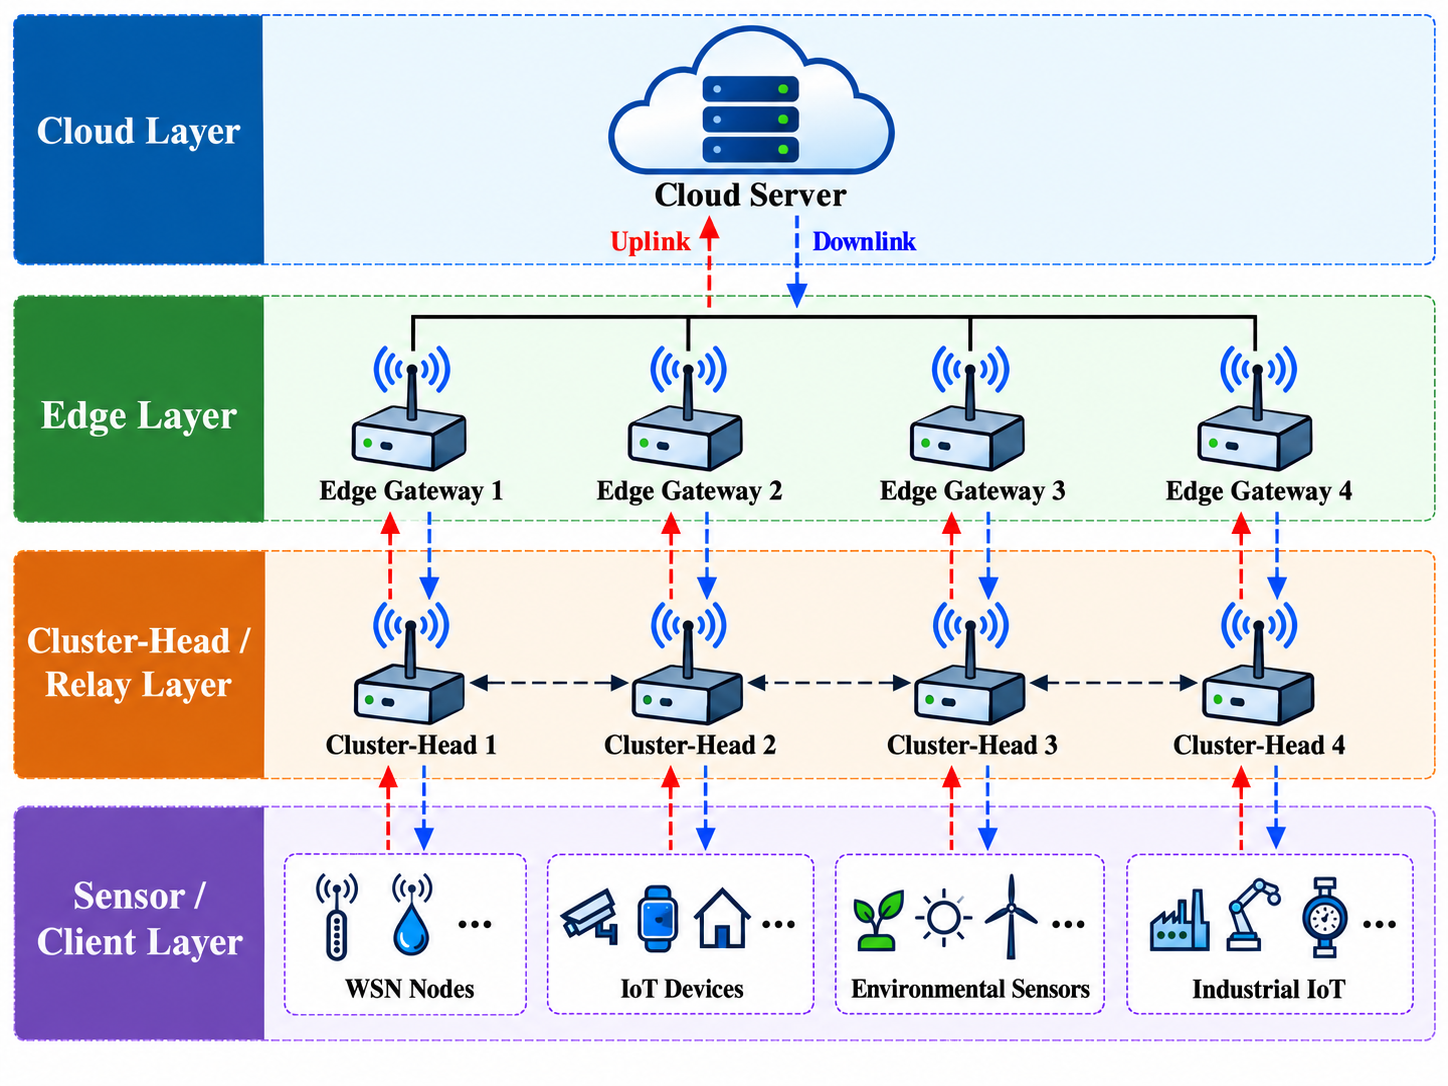
\includegraphics[width=0.96\linewidth]{figures/01_network_topology.png}
\caption{Intel Berkeley Lab WSN measured topology abstraction. Gateway motes are the configured edge gateways. Dashed links show a visually filtered subset of measured bidirectional-connectivity support; routing uses the full measured connectivity matrix and ETX values.}
\end{figure}
\subsection*{UCI Human Activity Recognition}
UCI HAR contains smartphone inertial features for 30 subjects and six activities [16]. Each subject is treated as a persistent FL client. Because the original benchmark separates subjects between train and test, the files are recombined before constructing per-subject local datasets. The original HAR windows overlap by 50\%; a random within-subject split can therefore leak overlapping signal content. The revised protocol preserves window order, partitions each subject record into contiguous 10-window blocks, assigns one of every five blocks to test using a deterministic subject-specific offset, and removes the immediately adjacent training window at each test boundary. This yields an approximately 80/20 overlap-safe within-client holdout. It is not the canonical unseen-subject UCI HAR benchmark.\par
\subsection*{Baselines and matched controls}
The core fixed-compression baselines are random, resource-only, and utility-only selection. To isolate the role of compression, random-adaptive, resource-adaptive, and utility-adaptive controls receive the same client-specific Top-k ratio rule as the proposed controller while retaining their original selection logic. The proposed-fixed-compression ablation applies the proposed selection rule at a fixed 50\% Top-k ratio.\par
The FedCG-adapted comparator uses current eligible-client gradient vectors in a greedy facility-location selection objective with a capability-cost penalty, followed by adaptive compression. Because this is a favorable adaptation with gradient access and because the original FedCG topology differs from the multi-hop HFL system, results are labeled FedCG-adapted rather than FedCG.\par
\subsection*{Metrics and statistical analysis}
Learning metrics are RMSE/MAE for Intel and accuracy/Macro-F1 plus worst-client and 10th-percentile accuracy for HAR. Systems metrics include expected transmitted bits, modeled local-plus-radio energy, maximum relay energy, residual energy, route hops, and ETX. Jain's index describes selection-frequency equality. Utility-target JS evaluates corrected cloud-influence alignment with the controller target. Temperature-coverage JS and class-coverage JS are independent distributional diagnostics.\par
Final real-data comparisons use exact paired sign-flip tests on the 10 held-out seeds, percentile bootstrap 95\% confidence intervals for paired mean differences, paired effect sizes, and Holm correction within each dataset-baseline metric family.\par
\subsection*{Control-plane signaling audit}
Network-aware selection requires pre-selection information, so a scheduler cannot legitimately treat all control metadata as free. We therefore add a conservative accounting-only audit. Each candidate reports one 168-bit (21-byte) packet per round: a 96-bit header, a 32-bit local-loss scalar, a 32-bit residual-energy estimate, and an 8-bit availability flag. The raw volume is T × N × 168 bits. To place metadata on the same basis as model updates, the audit multiplies each packet by that client's realized route ETX and sums over clients and rounds. A conservative radio-energy upper bound multiplies the ETX-weighted control bits by the sum of the configured Tx and Rx energy-per-bit coefficients. The audit is post-hoc: metadata energy is not fed back into residual energy or scheduling, so it cannot alter the reported learning trajectory.\par
The control-plane audit is intentionally stricter than a claim of negligible signaling. Its purpose is to test whether the adaptive-compression advantage survives when scheduler information is priced. It still excludes global-model downlink dissemination and therefore does not represent complete end-to-end device communication energy.\par
\subsection*{ns-3.47 communication replay}
Synthetic held-out traffic profiles are replayed in ns-3.47 LR-WPAN with CSMA/CA, acknowledgments, retries, and contention. The primary hop-equivalent mapping multiplies compressed update bits by mean selected hops and lets ns-3 generate its own MAC retransmissions. An ETX-equivalent mapping is retained as a stress sensitivity because ETX already contains expected transmission attempts. Five load/scaling conditions, four policies, two mappings, and 10 held-out seeds yield 400 ns-3 runs. The HFL optimizer itself is not executed inside ns-3.\par
\subsection*{Open-loop replay versus closed-loop co-simulation}
The current Python-to-ns-3 workflow is deliberately open loop. Python first completes the learning/controller trajectory and exports an offered-load profile; ns-3 then resolves MAC contention, acknowledgments, retries, delivery ratio, and packet delay. This design gives clean causal attribution from offered load to network behavior but does not permit packet outcomes to change future learning decisions. In a closed-loop co-simulation, packet drops or deadline misses would alter realized participation, stale updates would modify aggregation, measured retransmission energy would feed relay pressure, and updated link statistics could change subsequent routes and client selections. The present replay should therefore be interpreted as network-consequence validation rather than full cyber-physical co-simulation.\par
\subsection*{Reproducibility campaign}
The primary evaluation contains 240 tuning-grid HFL runs, 540 held-out real-data comparison runs, 100 held-out ablation runs, and 120 held-out synthetic runs: 1,000 HFL simulations in total, plus 400 ns-3 runs. The control-plane audit adds 40 accounting runs (proposed and proposed-fixed compression across the 10 held-out seeds on both real datasets). A regression test verifies two-level aggregation influence, and the frozen-table integrity checks are retained.\par
Repository verification is explicit rather than implicit. The tuning and held-out seed sets are defined in src/wsn\_hfl/config.py and mirrored in reproducibility/seed\_config.json; host hardware and the evidence boundary are documented in reproducibility/HARDWARE\_SPECIFICATIONS.md; reproduction commands are listed in reproducibility/REPRODUCTION\_COMMANDS.md; Tables 2 and 3 trace to the per-seed real-data outputs, aggregate summaries, and validation/statistics/statistical\_tests.csv; and the control-plane audit is reproduced by analyze\_control\_plane\_overhead.py. Dataset checksums, operating-point selection records, and frozen publication-table hashes are also committed.\par
\section{Results}
\subsection*{Synthetic stress test}
At correlation 0.9, held-out mean accuracy is 93.90\% for random, 94.12\% for resource-only, 93.93\% for utility-only, and 93.97\% for the proposed controller. The corresponding proposed effective traffic is 0.532 Mbit compared with 1.468 Mbit for resource-only. Utility-target JS is 0.0076 for proposed versus 0.0669 for resource-only. However, independent class-coverage JS is 0.00869 for proposed and 0.00728 for resource-only, reinforcing that target alignment and data-distribution coverage are different quantities.\par
\subsection*{Intel WSN held-out evaluation}
Table 2. Intel Berkeley Lab WSN results at correlation 0.9. Values are mean ± 95\% confidence interval over 10 held-out evaluation seeds.\par
\begin{table}[htbp]\centering\scriptsize
\resizebox{\linewidth}{!}{%
\begin{tabular}{lrrrrrrr}\toprule
Method & RMSE (°C)  & MAE (°C)  & Effective Mbit  & Energy (J)  & Max relay E (J)  & Utility-target JS  & Temp.-coverage JS  \\
\midrule
Resource & 1.7473 ± 0.0018 & 0.8369 ± 0.0048 & 2.230 ± 0.010 & 6.328 ± 0.022 & 0.1378 ± 0.0050 & 0.1057 ± 0.0045 & 0.00082 ± 0.00008 \\
Resource-adaptive & 1.7285 ± 0.0034 & 0.7638 ± 0.0114 & 0.916 ± 0.013 & 3.307 ± 0.031 & 0.0902 ± 0.0026 & 0.0843 ± 0.0044 & 0.00034 ± 0.00003 \\
FedCG-adapted & 1.7362 ± 0.0023 & 0.7903 ± 0.0065 & 0.980 ± 0.013 & 3.454 ± 0.030 & 0.0964 ± 0.0016 & 0.0911 ± 0.0033 & 0.00027 ± 0.00003 \\
Proposed-fixed 50\% & 1.7369 ± 0.0029 & 0.8048 ± 0.0080 & 2.373 ± 0.010 & 6.658 ± 0.022 & 0.1430 ± 0.0047 & 0.0283 ± 0.0023 & 0.00258 ± 0.00021 \\
Proposed & 1.7348 ± 0.0030 & 0.7790 ± 0.0060 & 0.992 ± 0.021 & 3.482 ± 0.049 & 0.0969 ± 0.0024 & 0.0118 ± 0.0013 & 0.00375 ± 0.00019 \\
\bottomrule\end{tabular}}
\end{table}
\begin{figure}[htbp]
\centering
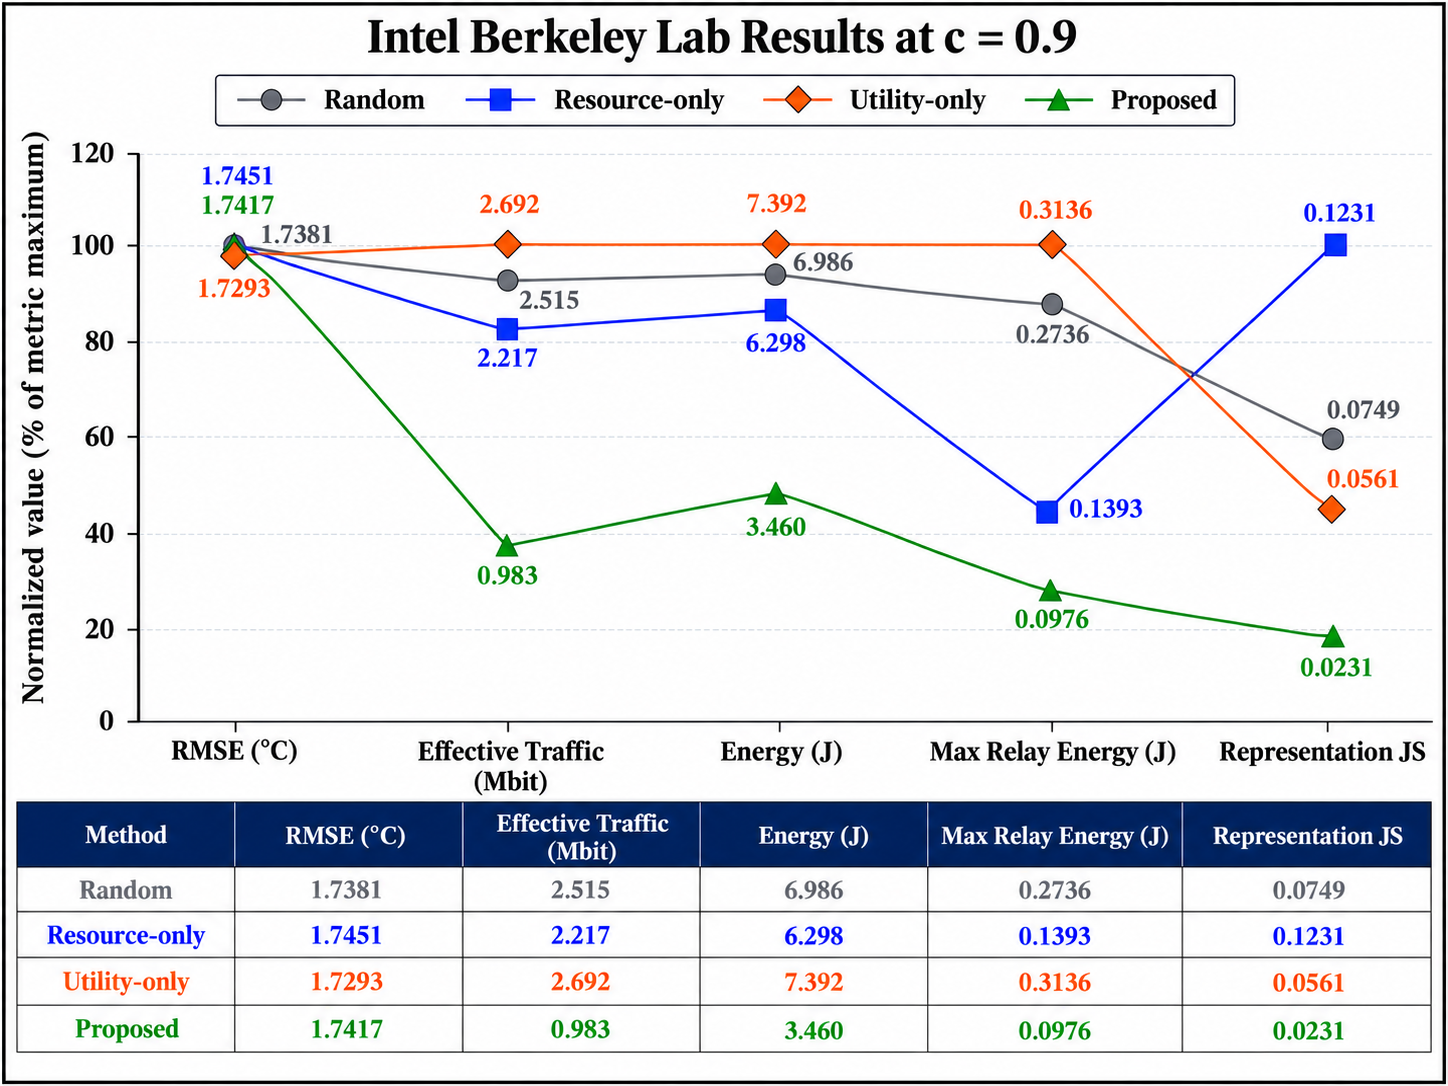
\includegraphics[width=0.96\linewidth]{figures/07_intel_berkeley_results.png}
\caption{Intel held-out evaluation at c = 0.9. Raw means are annotated and tabulated. The line plot normalizes each metric to its own within-metric maximum only for visual comparison; it is not a composite performance score. Confidence intervals are reported in Table 2.}
\end{figure}
Relative to the fixed-compression resource baseline, the proposed controller reduces traffic by 55.5\% and modeled energy by 45.0\%, but the matched resource-adaptive control shows that those headline savings cannot be attributed to scheduling alone. Resource-adaptive uses 8.3\% less traffic and 5.3\% less modeled energy than proposed and obtains lower RMSE and MAE. The proposed controller instead reduces utility-target JS by 86.0\% relative to resource-adaptive. Its temperature-coverage JS is worse, not better. Against FedCG-adapted, RMSE, traffic, energy, and maximum relay energy are statistically comparable after Holm correction, while utility-target JS is 87.1\% lower. This result supports a target-alignment trade-off rather than statistical-representativeness superiority.\par
\subsection*{UCI HAR held-out evaluation}
Table 3. UCI HAR results at correlation 0.9 using the overlap-safe blocked within-client holdout. Values are mean ± 95\% confidence interval over 10 held-out evaluation seeds.\par
\begin{table}[htbp]\centering\scriptsize
\resizebox{\linewidth}{!}{%
\begin{tabular}{lrrrrrrrr}\toprule
Method & Accuracy  & Macro-F1  & Worst-client acc.  & Effective Mbit  & Energy (J)  & Max relay E (J)  & Utility-target JS  & Class-coverage JS  \\
\midrule
Resource & 0.8641 ± 0.0114 & 0.8565 ± 0.0140 & 0.5467 ± 0.0227 & 28.785 ± 0.898 & 44.73 ± 1.44 & 0.459 ± 0.088 & 0.1716 ± 0.0207 & 0.000081 ± 0.000032 \\
Resource-adaptive & 0.8751 ± 0.0047 & 0.8698 ± 0.0057 & 0.5567 ± 0.0254 & 8.872 ± 0.363 & 14.34 ± 0.57 & 0.170 ± 0.036 & 0.1553 ± 0.0203 & 0.000075 ± 0.000038 \\
FedCG-adapted & 0.8760 ± 0.0033 & 0.8705 ± 0.0041 & 0.5367 ± 0.0270 & 9.311 ± 0.389 & 15.34 ± 0.65 & 0.643 ± 0.135 & 0.1341 ± 0.0199 & 0.000070 ± 0.000024 \\
Proposed-fixed 50\% & 0.7947 ± 0.0253 & 0.7570 ± 0.0392 & 0.5032 ± 0.0512 & 31.232 ± 1.001 & 49.26 ± 1.98 & 0.807 ± 0.322 & 0.1010 ± 0.0191 & 0.000078 ± 0.000020 \\
Proposed & 0.8867 ± 0.0012 & 0.8827 ± 0.0011 & 0.5683 ± 0.0294 & 11.253 ± 0.352 & 19.20 ± 0.75 & 1.242 ± 0.275 & 0.0275 ± 0.0034 & 0.000064 ± 0.000018 \\
\bottomrule\end{tabular}}
\end{table}
\begin{figure}[htbp]
\centering
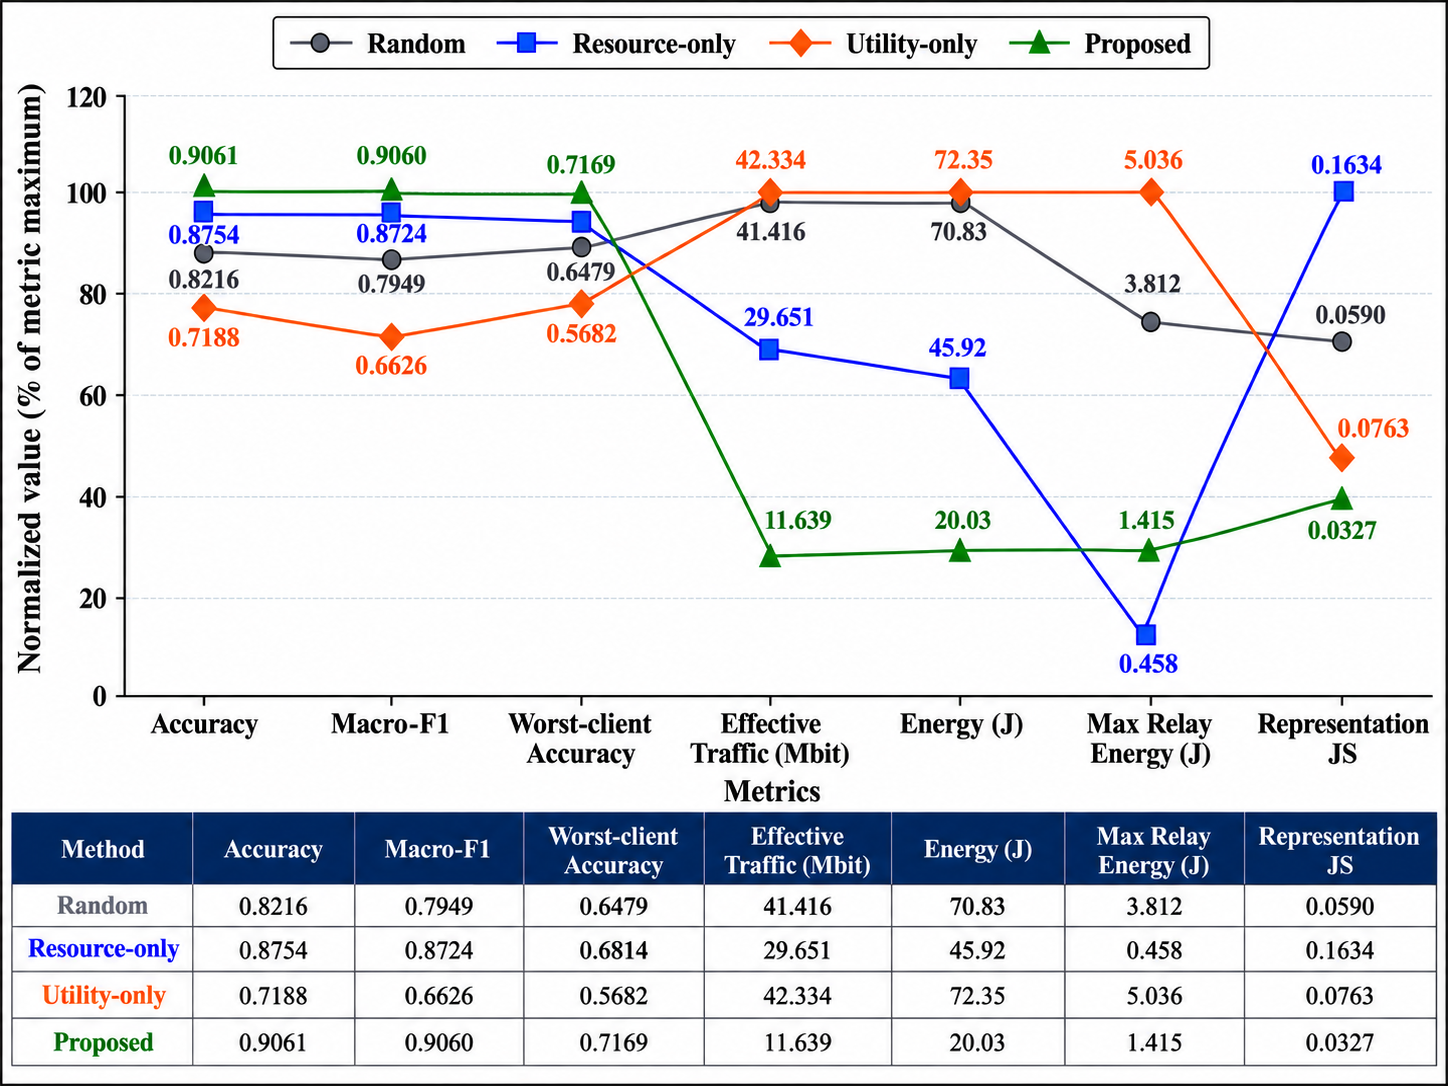
\includegraphics[width=0.96\linewidth]{figures/06_uci_har_results.png}
\caption{UCI HAR held-out evaluation at c = 0.9 using the blocked overlap-safe within-client split. Raw means are annotated and tabulated. The line plot uses within-metric normalization only for visualization; it is not a composite score. Confidence intervals are reported in Table 3.}
\end{figure}
The proposed controller improves held-out accuracy by 1.16 percentage points over resource-adaptive and by 1.07 points over FedCG-adapted; both differences remain significant after Holm correction. The gain is purchased with additional network cost: relative to resource-adaptive, proposed traffic increases 26.8\%, modeled energy 33.9\%, and maximum relay energy 628.9\%. Against FedCG-adapted, traffic increases 20.9\%, energy 25.1\%, and maximum relay energy 93.0\%. Utility-target JS is 82.3\% lower than resource-adaptive and 79.5\% lower than FedCG-adapted. In contrast, class-coverage JS differences are small and non-significant. This is exactly the distinction intended by the revised metric terminology.\par
\subsection*{Compression and component ablations}
On Intel, adaptive fidelity reduces proposed traffic from 2.373 Mbit at fixed 50\% compression to 0.992 Mbit, a 58.2\% reduction, and modeled energy falls by 47.7\%; RMSE changes only from 1.7369 to 1.7348 °C. Removing the participation-deficit queue increases utility-target JS from 0.0118 to 0.0318. Removing relay pressure increases maximum relay energy from 0.0969 J to 0.1062 J.\par
On HAR, adaptive fidelity reduces proposed traffic from 31.232 Mbit to 11.253 Mbit, a 64.0\% reduction, and energy falls from 49.26 J to 19.20 J. Accuracy simultaneously rises from 79.47\% to 88.67\% because the fixed-compression traffic incurs larger latency/staleness and dropout consequences in the modeled system. Removing the participation-deficit queue lowers network cost but increases utility-target JS from 0.0275 to 0.0854 and reduces accuracy from 88.67\% to 88.39\%. Removing relay pressure lowers utility-target JS but raises maximum relay energy from 1.242 J to 1.599 J, illustrating that individual terms can improve one objective while worsening another.\par
\begin{figure}[htbp]
\centering
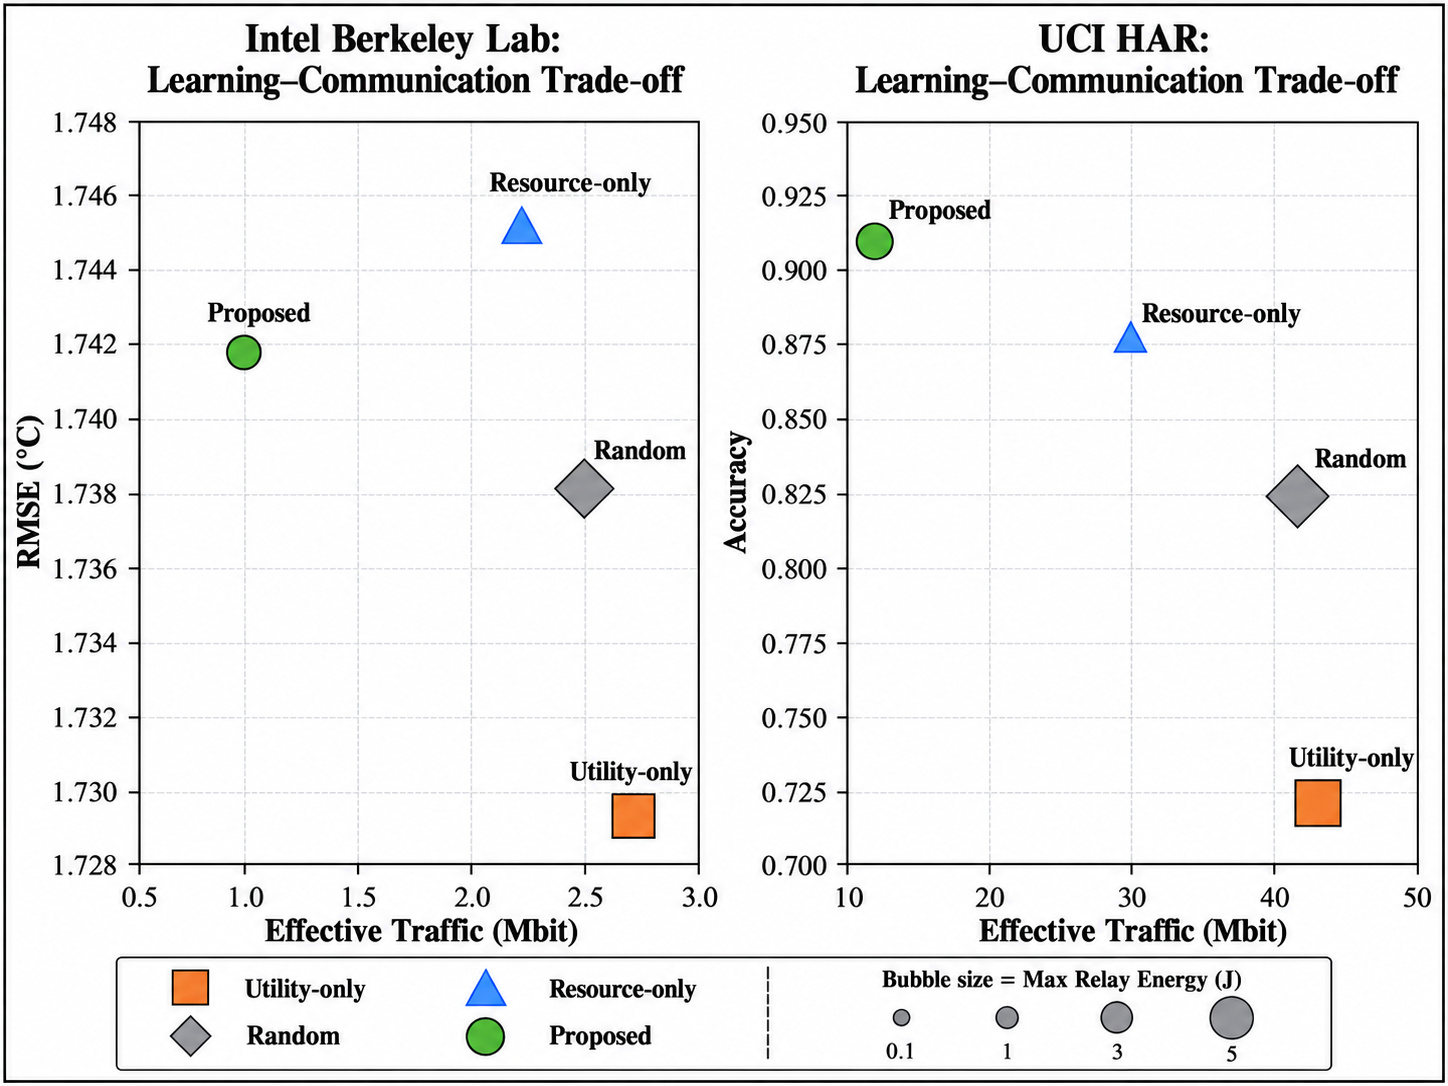
\includegraphics[width=0.96\linewidth]{figures/04_ablation.png}
\caption{Held-out component ablations on Intel and UCI HAR at c = 0.9. 'No deficit' removes the utility-target participation-deficit term. Adaptive fidelity is the principal source of traffic reduction, while relay pressure and participation deficit affect different trade-off dimensions.}
\end{figure}
\subsection*{Control-plane overhead audit}
The control-plane result is workload dependent rather than universally negligible. On Intel, 48 learning clients over 30 rounds generate 241,920 raw metadata bits (29.53 KiB). ETX weighting increases the held-out mean to 1.219 Mbit, with a conservative metadata radio-energy upper bound of 2.803 J. This is 122.8\% of the proposed controller's 0.992 Mbit compressed model-update traffic, so control signaling is material for the small regression model.\par
On HAR, 30 clients over 25 rounds generate 126,000 raw metadata bits (15.38 KiB). The ETX-weighted mean is 0.306 Mbit with a 0.705 J conservative radio-energy upper bound, only 2.72\% of the proposed 11.253 Mbit model-update traffic.\par
Table 4. Conservative pre-selection metadata audit at correlation 0.9. Values are means over 10 held-out evaluation seeds.\par
\begin{table}[htbp]\centering\scriptsize
\resizebox{\linewidth}{!}{%
\begin{tabular}{lrrrrrrr}\toprule
Dataset & Raw metadata & ETX-weighted metadata (Mbit) & Metadata radio-energy upper bound (J) & Metadata / proposed model traffic & Proposed control-inclusive uplink (Mbit) & Proposed-fixed control-inclusive uplink (Mbit) & Adaptive reduction after metadata \\
\midrule
Intel & 29.53 KiB & 1.219 & 2.803 & 122.8\% & 2.211 & 3.592 & 38.4\% \\
UCI HAR & 15.38 KiB & 0.306 & 0.705 & 2.72\% & 11.559 & 31.539 & 63.3\% \\
\bottomrule\end{tabular}}
\end{table}
Thus metadata does not erase the adaptive-fidelity advantage, but it materially changes the size of that advantage for lightweight models. The correct claim is therefore that control overhead is small relative to model traffic for HAR but not for Intel. Even under the conservative all-client-per-round accounting model, proposed adaptive fidelity retains a 38.4\% control-inclusive uplink reduction on Intel and 63.3\% on HAR relative to the same proposed selector at fixed 50\% Top-k. These totals still exclude downlink global-model dissemination.\par
\subsection*{ns-3 communication replay}
Under the primary hop-equivalent dense-nominal condition, proposed held-out synthetic traffic maps to 1,204 payload bits per report-equivalent update, compared with 3,431 for resource-only. The mean report delivery ratio is 99.47\% for proposed and 85.79\% for resource-only; mean delivered-report delay is 12.26 ms versus 35.99 ms. At the 24-sensor scale-nominal condition, report delivery is 96.56\% for proposed versus 57.72\% for resource-only. These differences establish a narrower but operationally important result: lower offered load survives translation into a contention-aware IEEE 802.15.4 network and materially changes delivery, delay, and access failures. They do not independently prove superiority of the learning scheduler, because the replay is open loop and packet outcomes do not feed back into future client selection. The traffic reduction itself is strongly influenced by adaptive compression.\par
\begin{figure}[htbp]
\centering
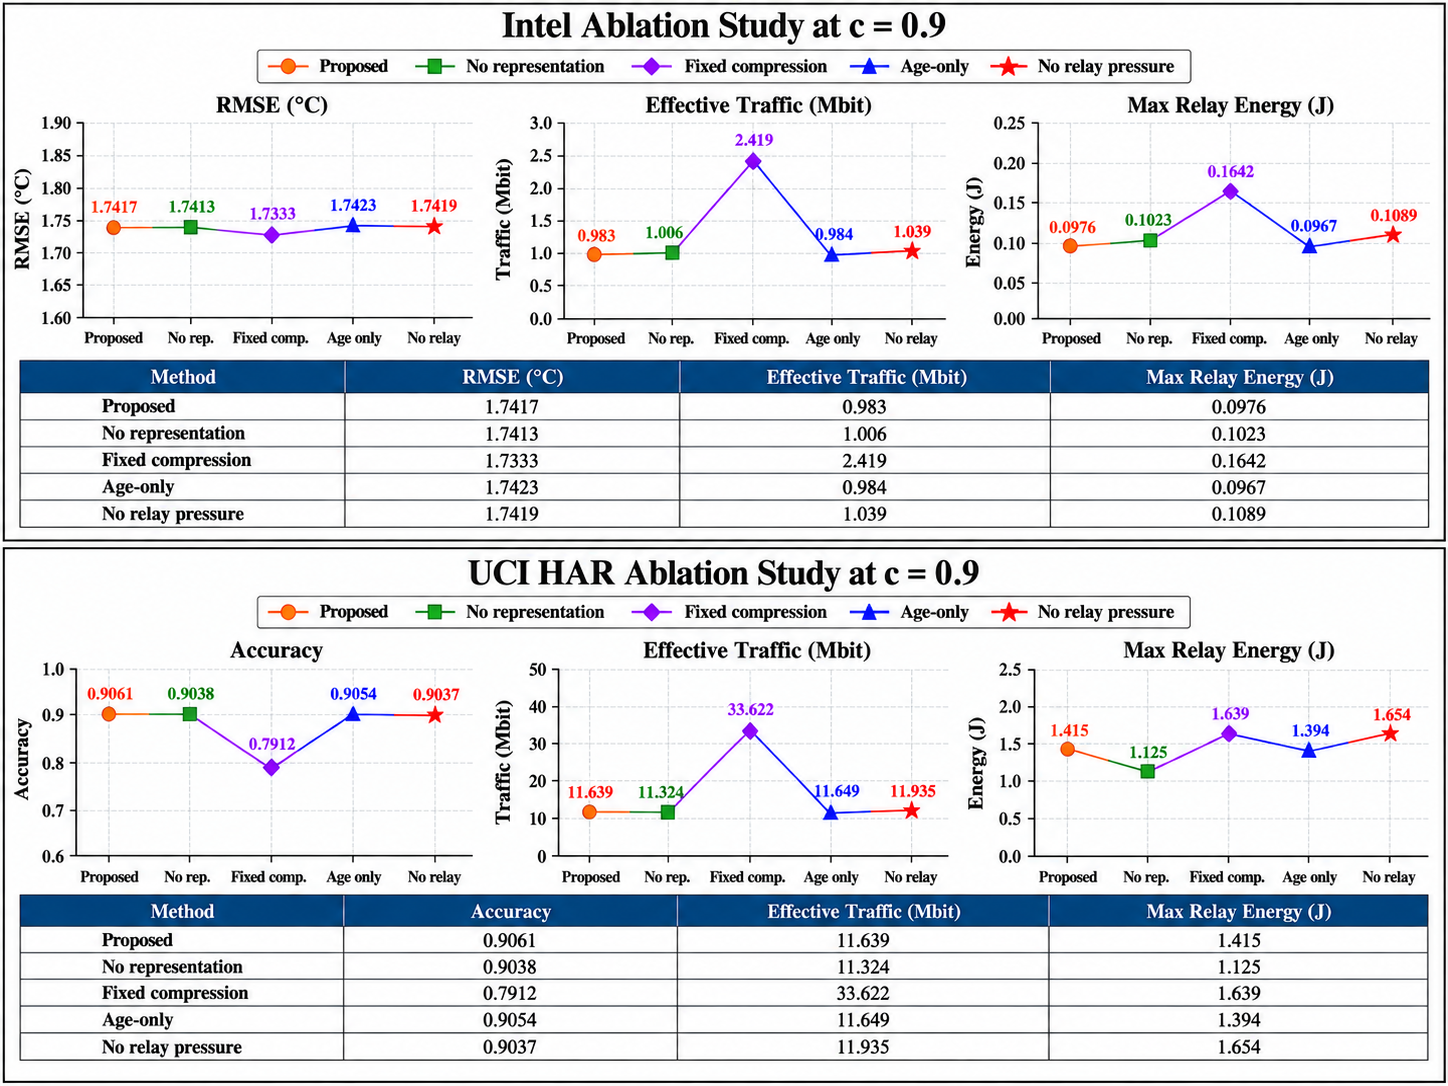
\includegraphics[width=0.96\linewidth]{figures/03_ns3_validation.png}
\caption{ns-3.47 IEEE 802.15.4/LR-WPAN hop-equivalent replay of held-out synthetic traffic. Report delivery ratio, delivered-report delay, and channel-access failures are shown for dense-nominal and 24-sensor-nominal conditions. The HFL controller itself is not executed inside ns-3.}
\end{figure}
\subsection*{Cross-dataset interpretation}
The held-out results reject a simple “best method” interpretation and instead expose two different Pareto regimes. On Intel, resource-adaptive provides the stronger prediction/resource operating point, with lower error, traffic, energy, and relay burden, while proposed most closely matches its own utility-derived target. FedCG-adapted is statistically comparable to proposed on Intel RMSE and systems cost. On HAR, proposed improves held-out accuracy from 87.51\% to 88.67\% relative to resource-adaptive, but model-update traffic rises by 26.8\%, modeled energy by 33.9\%, and maximum relay energy by 628.9\%. Against FedCG-adapted, the accuracy advantage is 1.07 percentage points with 20.9\% more model-update traffic and 93.0\% more maximum relay energy. These are not hidden implementation penalties; they are the physical price of prioritizing utility-target participation and learning quality in this operating regime. Independent coverage metrics do not mirror utility-target JS, confirming that target alignment is not equivalent to representativeness.\par
\begin{figure}[htbp]
\centering
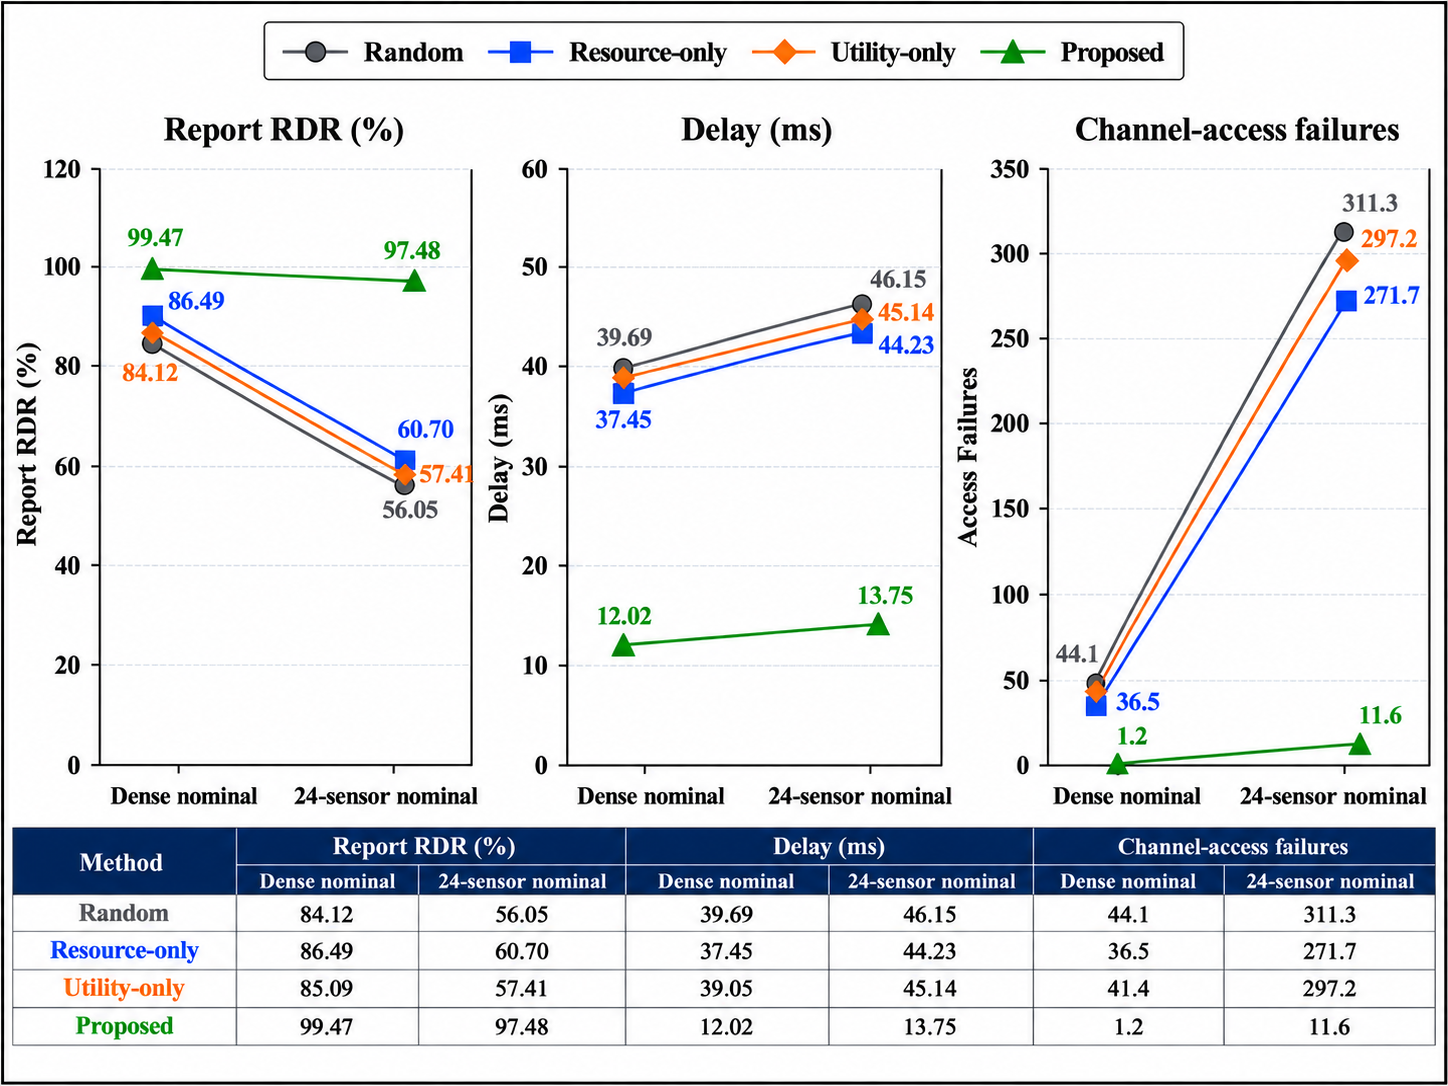
\includegraphics[width=0.96\linewidth]{figures/05_learning_communication_tradeoff.png}
\caption{Held-out learning-versus-uplink-model-update-traffic trade-offs at c = 0.9. Marker area scales with maximum relay energy. The figure includes compression-matched controls, the FedCG-adapted comparator, and the proposed controller.}
\end{figure}
The practical design implication is that a deployment should choose an operating point according to the objective it actually values. A relay-lifetime-constrained deployment can legitimately prefer resource-adaptive, whereas an application with a stricter prediction requirement may accept the additional network burden of the proposed HAR operating point. The contribution is therefore the ability to expose and control this exchange rather than collapse competing objectives into a claim of universal superiority.\par
Adaptive fidelity and client scheduling should also be evaluated separately. A fixed-compression baseline can make a coupled controller appear dramatically more communication-efficient even when most of the reduction comes from the compression rule. Conversely, a pure resource controller can minimize traffic and hotspot energy while accepting weaker alignment with the utility target. The revised evaluation makes these trade-offs explicit.\par
\section{Discussion}
\subsection*{Evidence hierarchy: exact analysis and executable systems behavior}
The strongest evidence from the revision is the separation between what can be established exactly for the implemented decision rules and what must be tested in an executable network. Corrected two-level influence accounting materially changes the interpretation of the JS metric: it is now the true cloud coefficient accumulated across the hierarchy, but it remains an endogenous utility-target diagnostic. Disjoint tuning and held-out seeds prevent parameter-selection outcomes from being reused as inferential evidence, while compression-matched controls show that adaptive update fidelity is the principal source of the large model-traffic reductions.\par
A systems-learning controller should not be judged exclusively through a convergence-rate lens. Smooth or convex surrogate analyses can isolate optimization behavior, but packet contention, retransmissions, finite-set sparsification, route changes, and asynchronous arrival are the mechanisms that determine feasibility in a resource-bounded edge system. The present approach therefore uses analytical results where they apply exactly and executable evidence where the physical abstraction matters. The queue identities and finite-set decisions establish controller-level properties; real sensing data and ns-3 replay expose consequences that disappear when communication is reduced to a differentiable scalar penalty. These forms of evidence are complementary rather than interchangeable.\par
\subsection*{Model-complexity scaling}
The current experiments deliberately use lightweight predictors so that orchestration effects can be isolated. Moving to a 1D-CNN, MobileNet-like TinyML model, or another nonlinear edge architecture changes both communication volume and local compute cost. If a model contains P trainable parameters and retains fraction rho under index-based Top-k transmission, the approximate sparse payload is 96 + ceil(rho P)(32 + 16) bits under the present value/index accounting. Ignoring the fixed header, sparse transmission is smaller than a dense 32-bit update only when rho < 2/3. A scalable implementation should therefore switch between sparse and dense encodings rather than attach a 16-bit index to every retained coordinate when rho is large.\par
Model size also changes the transmission-to-computation energy ratio. Architectures with high arithmetic intensity can move the system toward compute-dominated energy, whereas large parameter tensors with modest compute intensity can remain communication dominated. Deep models additionally exhibit layer-dependent update scales, so global Top-k may over-select coordinates from high-magnitude layers; layer-wise sparsification, structured sparsity, or joint quantization can become preferable. The present experiments establish the orchestration mechanism for lightweight edge models, not the same communication-computation optimum for every TinyML architecture.\par
\subsection*{Pareto interpretation across workloads}
Intel and HAR occupy different Pareto regimes. Intel shows that resource-adaptive can simultaneously provide lower error and lower systems cost, whereas the proposed controller buys substantially stronger utility-target alignment. HAR reverses part of that ordering: proposed improves held-out accuracy by about one percentage point over resource-adaptive and FedCG-adapted, but at materially higher traffic and relay cost. This cross-dataset reversal is a useful systems result because it shows why no fixed orchestration principle dominates across sensing workloads.\par
The broader relevance to resource-bounded edge intelligence is consequently not a claim that the current simulator proves environmental sustainability. Rather, it demonstrates how learning objectives can be audited together with the network externalities they impose. Environmental monitoring, infrastructure sensing, and wearable activity systems all face variants of this coupling, but deployment-specific hardware measurements remain necessary before modeled joules are translated into battery lifetime or sustainability outcomes.\par
\section{Limitations}
First, energy is modeled rather than measured on physical IEEE 802.15.4 sensor hardware. No claim is made about MCU current draw, radio current, RSSI/LQI, battery lifetime, embodied energy, or environmental sustainability. Second, Intel uses historical measured connectivity and sensing traces; the original motes do not execute the FL process. Third, the HAR protocol is a blocked within-client holdout designed for subject-as-client FL and should not be compared directly with the canonical unseen-subject benchmark.\par
Fourth, the utility target is controller defined. Low utility-target JS proves alignment with that target, not independent population representativeness. Fifth, the new control-plane audit prices all-client pre-selection metadata, but it remains an accounting diagnostic rather than a closed-loop energy charge. Global-model downlink dissemination is still excluded, and reported control-inclusive values therefore remain uplink-side rather than complete device communication energy. Event-triggered, eligibility-gated, or piggybacked metadata could substantially reduce the Intel control burden but is not implemented here.\par
Sixth, the ns-3 workflow is open loop. The replay resolves contention, retries, delivery, and delay after the learning trajectory has already been generated; packet drops do not cause future client timeouts, route changes, or altered queue evolution. Closed-loop Python-ns-3 co-simulation remains a stronger future validation target.\par
Seventh, FedCG-adapted is not an exact reimplementation of FedCG. It uses a gradient-diversity facility-location principle and adaptive compression under the current candidate pool, but the original algorithm's topology and optimization assumptions differ. The comparator also receives current eligible-client gradients without charging their acquisition cost, making it a deliberately favorable reference rather than an unfairly weak baseline.\par
Eighth, local predictors are linear and intentionally lightweight. Larger TinyML models may alter computation, sparsification sensitivity, update geometry, and the relative value of communication savings. Ninth, the relay virtual queue uses a reference level rather than enforcing a hard prospective energy cap; the HAR result demonstrates that hotspot energy can still become large when the controller prioritizes learning/target objectives. Finally, the theory establishes finite-horizon queue bounds, finite-set compression optimality, top-k score optimality, and error-feedback conservation, but not a complete non-convex convergence theorem for the coupled selection-compression-hierarchy-network process.\par
\section{Conclusion}
This work reframes network-aware federated learning as an energy-information co-design problem for resource-bounded edge intelligence. The central systems question is not simply how to reduce model traffic, but how to allocate scarce communication and relay resources without disconnecting learning decisions from the value and timing of distributed information.\par
The proposed controller exposes route burden, residual-energy scarcity, relay pressure, participation deficit, update fidelity, and staleness to a common orchestration layer. A stricter experimental protocol reveals that this coupling does not generate universal dominance. On Intel, resource-adaptive provides a stronger prediction/resource operating point, whereas the proposed policy achieves substantially closer utility-target alignment. On HAR, the proposed controller improves held-out accuracy but does so at substantial relay-energy and communication cost. These reversals are a principal finding rather than a weakness: they demonstrate that resource-bounded distributed AI is intrinsically Pareto constrained.\par
Adaptive update fidelity remains the dominant mechanism behind the observed model-traffic reductions. Importantly, the control-plane audit shows that metadata cannot always be treated as free. Signaling is small relative to HAR model traffic but material for the lightweight Intel model; nevertheless, adaptive fidelity retains a 38.4\% control-inclusive uplink traffic reduction on Intel and 63.3\% on HAR relative to the same proposed scheduler at fixed 50\% Top-k.\par
Finally, ns-3.47 replay establishes that reduced offered load produces measurable packet-network benefits under contention while also defining the boundary of the evidence: replay is open loop and does not yet allow packet outcomes to alter future learning decisions. Closed-loop packet/learning co-simulation and nonlinear TinyML architectures are therefore the next steps toward experimentally grounded resource-aware distributed intelligence.\par
\section{Author contributions}
All authors contributed equally to the conceptualization, methodology, investigation, validation, formal analysis, interpretation of results, manuscript preparation, critical revision, and final approval of the work.\par
\section{Funding}
This research received no external funding.\par
\section{Declaration of interests}
The authors declare no competing interests.\par
\section{Declaration of generative AI and AI-assisted technologies in the writing process}
During the preparation of this manuscript, the authors used OpenAI ChatGPT to support literature-review organization and language editing. The tool was not treated as an evidence source and was not used to replace author verification of citations, data, analyses, or conclusions. All AI-assisted material was critically reviewed, verified, and edited by the authors, who take full responsibility for the accuracy, integrity, citations, and final content of the manuscript.\par
\section*{Resource availability}
\subsection*{Lead contact}
Requests concerning the manuscript should be directed to the corresponding author, Abhishek Kumar Pandey (abhishek.pandey2@bennett.edu.in).\par
\subsection*{Materials availability}
This computational study did not generate new physical materials.\par
\subsection*{Data and code availability}
Code, experiment manifests, tuning and held-out seed lists, raw per-seed outputs, statistical analyses, control-plane audit outputs, and the seven user-verified manuscript figures are available in the public project repository: https://github.com/DrShivamBhardwaj/Relevance\_Aware\_RE\_ETX\_/tree/wsn-hfl-crosslayer-final. Intel Berkeley Lab sensor data and UCI HAR are publicly available from their original providers. The repository records the operating-point selection rule, corrected hierarchical-influence test, seed configuration, host-hardware specification, reproduction commands, and SHA-256 hashes that lock the approved final figure set.\par
\section*{References}
\noindent [1] L. Liu, J. Zhang, S. H. Song, and K. B. Letaief, “Client-Edge-Cloud Hierarchical Federated Learning,” IEEE International Conference on Communications, 2020. DOI: 10.1109/ICC40277.2020.9148862.\par
\noindent [2] S. AbdulRahman, H. Tout, A. Mourad, and C. Talhi, “FedMCCS: Multicriteria Client Selection Model for Optimal IoT Federated Learning,” IEEE Internet of Things Journal, 8, 4723–4735, 2021. DOI: 10.1109/JIOT.2020.3028742.\par
\noindent [3] W. Y. B. Lim, J. S. Ng, Z. Xiong, D. Niyato, C. Miao, and D. I. Kim, “Dynamic Edge Association and Resource Allocation in Self-Organizing Hierarchical Federated Learning Networks,” IEEE Journal on Selected Areas in Communications, 39(12), 3640–3653, 2021. DOI: 10.1109/JSAC.2021.3118401.\par
\noindent [4] T. Huang, W. Lin, L. Shen, K. Li, and A. Y. Zomaya, “Stochastic Client Selection for Federated Learning With Volatile Clients,” IEEE Internet of Things Journal, 9(20), 20055–20070, 2022. DOI: 10.1109/JIOT.2022.3172113.\par
\noindent [5] X. Chen, T. Ouyang, Z. Zhou, X. Zhang, S. Yang, and J. Zhang, “HiFlash: Communication-Efficient Hierarchical Federated Learning With Adaptive Staleness Control and Heterogeneity-Aware Client-Edge Association,” IEEE Transactions on Parallel and Distributed Systems, 2023. DOI: 10.1109/TPDS.2023.3238049.\par
\noindent [6] Z. Jiang, Y. Xu, H.-Z. Xu, Z. Wang, and C. Qian, “Heterogeneity-Aware Federated Learning with Adaptive Client Selection and Gradient Compression,” IEEE INFOCOM, 2023. DOI: 10.1109/INFOCOM53939.2023.10229029.\par
\noindent [7] Y. Deng, F. Lyu, T. Xia, Y. Zhou, Y. Zhang, J. Ren, and Y. Yang, “A Communication-Efficient Hierarchical Federated Learning Framework via Shaping Data Distribution at Edge,” IEEE/ACM Transactions on Networking, 32(3), 2600–2615, 2024. DOI: 10.1109/TNET.2024.3363916.\par
\noindent [8] B. Wu, F. Fang, X. Wang, D. Cai, S. Fu, and Z. Ding, “Client Selection and Cost-Efficient Joint Optimization for NOMA-Enabled Hierarchical Federated Learning,” IEEE Transactions on Wireless Communications, 23(10), 14289–14303, 2024. DOI: 10.1109/TWC.2024.3411479.\par
\noindent [9] X. Chen, G. Zhu, Y. Deng, and Y. M. Fang, “Federated Learning Over Multihop Wireless Networks With In-Network Aggregation,” IEEE Transactions on Wireless Communications, 2022. DOI: 10.1109/TWC.2022.3168538.\par
\noindent [10] P. Pinyoanuntapong, P. Janakaraj, R. Balakrishnan, M. Lee, C. Chen, and P. Wang, “EdgeML: Towards Network-Accelerated Federated Learning over Wireless Edge,” Computer Networks, 218, 109396, 2022. DOI: 10.1016/j.comnet.2022.109396.\par
\noindent [11] T. V. Nguyen, N. D. Ho, H. T. Hoang, C. D. Do, and K.-S. Wong, “Toward Efficient Hierarchical Federated Learning Design Over Multi-Hop Wireless Communications Networks,” IEEE Access, 10, 111910–111922, 2022. DOI: 10.1109/ACCESS.2022.3215758.\par
\noindent [12] J. Wu, F. Dong, H. Leung, Z. Zhu, J. Zhou, and S. Drew, “Topology-Aware Federated Learning in Edge Computing: A Comprehensive Survey,” ACM Computing Surveys, 56(10), Article 262, 1–41, 2024. DOI: 10.1145/3659205.\par
\noindent [13] M. Alsofyani, I. Al-Turaiki, and H. Mathkour, “A Fairness Perspective on Client Selection and Aggregation Methods for Non-IID Mitigation in Federated Learning: A Survey,” Electronics, 2026. DOI: 10.3390/electronics15143178.\par
\noindent [14] M. J. Neely, Stochastic Network Optimization with Application to Communication and Queueing Systems, Morgan \& Claypool, 2010. DOI: 10.2200/S00271ED1V01Y201006CNT007.\par
\noindent [15] Intel Berkeley Research Lab sensor dataset. Available: https://db.csail.mit.edu/labdata/labdata.html.\par
\noindent [16] UCI Machine Learning Repository, “Human Activity Recognition Using Smartphones.” DOI: 10.24432/C54S4K.\par
\noindent [17] E. Yu, S. Liu, Q. Li, H. Chen, H. V. Poor, and S. Shamai, “Graph-Based Joint Client Clustering and Resource Allocation for Wireless Distributed Learning: A New Hierarchical Federated Learning Framework With Non-IID Data,” IEEE Transactions on Mobile Computing, 24(5), 3579–3596, 2025. DOI: 10.1109/TMC.2024.3515037.\par
\noindent [18] M. Wu, M. Boban, and F. Dressler, “Hierarchical Federated Learning in Device-to-Device Networks With Learning-Topology Co-Optimization,” IEEE Transactions on Mobile Computing, 25(8), 12488–12505, 2026. DOI: 10.1109/TMC.2026.3673393.\par
\noindent [19] W. Hu, Y. Yu, X. Hao, X. Cai, Y. Qian, L. Guo, and Y. Li, “Multi-Job Hierarchical Federated Learning for Consumer-Grade UAVs: A Joint Client Selection and Resource Allocation Approach,” IEEE Transactions on Consumer Electronics, 71(3), 8021–8032, 2025. DOI: 10.1109/TCE.2025.3587021.\par
\noindent [20] “Joint Communication and Computing Resource Allocation for Energy Efficient Hierarchical Federated Learning in Marine Internet of Things,” IEEE Transactions on Network Science and Engineering, 12(5), 4114–4127, 2025. DOI: 10.1109/TNSE.2025.3568875.\par
\end{document}